

\section{\todo{Мобильный робот в форме эллипсоида}}

\begin{frame}[plain, noframenumbering]
	\begin{center}
		\Huge
		\todo{Мобильный робот в форме эллипсоида}
	\end{center}
\end{frame}

\begin{frame}
\frametitle{Конструкция}
Конструкция и корпусные элементы экспериментальной модели безвинтового подводного робота
\begin{figure}[h]
	\centering
	\includegraphics[width=0.7\linewidth]{constr_BPR.png}%		
\end{figure}
Фотографии робота в сборе и без половины оболочки
\begin{figure}[h]
	\centering
	\includegraphics[width=0.8\linewidth]{Photo_BPR.png}%
\end{figure}

\end{frame}


\small
\begin{frame}%[allowframebreaks]
	\frametitle{Математическая модель}
		\qquad Рассмотрим систему, состоящую из жесткой внешней оболочки и трех внутренних роторов. \todo{Нарисовать свой рисунок}
		
		\begin{figure}[h]
			\begin{center}
				\includegraphics[width=0.4\linewidth]{BPR_Scheme.png}
				
			\end{center}
		\end{figure}		
		
		\begin{itemize}
			% \item Оболочка является однородной, положение ее центра масс совпадает с геометрическим центром оболочки.
			% \item Центр масс всей системы находится не в геометрическом центре оболочки;
			% \item Все роторы одинаковы, осесимметричны и оси вращения  совпадают с их осями симметрии, то есть вращение не изменяет распределение масс системы;
			%\item Ось вращения одного из роторов совпадает с осью винтовой симметрии оболочки;
			% \item Оси вращения роторов взаимно перпендикулярны, а их угловые скорости являюся заданными функциями времени $\omega _k \bigl( t \bigr),~k=1,2,3$.
			
			%\framebreak
			
			\item $O_M e_1 e_2 e_3$ -- подвижная система координат, жестко связанная с оболочкой, так что оси совпадают с главными осями инерции оболочки.
			
			% \item $\bV$ и ${\bOm}$ -- скорость центра оболочки и его угловую скорость.
			
			\item $O x y z$ -- неподвижная система координат; 
			$\br = \bigl( x,\, y,\, z \bigr)$ -- координаты геометрического центра оболочки в этих осях. %${\bal}$, ${\bbe}$, ${\bga}$ -- орты неподвижных осей $O x y z$, спроецированные на подвижные оси $e_1$, $e_2$, $e_3$, тогда ортогональная матрица
%			\begin{gather}
%			\bbQ =\begin{pmatrix}
%			\alpha _1 & \beta _1 & \gamma _1\\
%			\alpha _2 & \beta _2 & \gamma _2\\
%			\alpha _3 & \beta _3 & \gamma _3
%			\end{pmatrix}\nonumber \in SO(3)
%			\end{gather}
%			
%			характеризует ориентацию тела.
			
			% \item Пара $\left( \br,\, \bm{Q} \right)$ однозначно определяет конфигурацию системы. 
			
			%\item Конфигурационное пространство системы шестимерно и представляет собой $\mathbb{R}^3 \times SO(3)$.
		\end{itemize}
\end{frame}

%\begin{frame}
%\frametitle{Математическая модель}
%	\begin{itemize}
%	
%	\end{itemize}
%\end{frame}

\begin{frame}
	\frametitle{Математическая модель}
	\begin{itemize}
		\item Кинетическая энергия оболочки:
		\begin{gather}
		T_s = \frac{1}{2} m_s  \bigl( \bV,\, \bV \bigr) + \frac{1}{2} \bigl( {\bm I}_s {\bOm},\, {\bOm} \bigr),\nonumber
		\end{gather}
	
		\item Кинетическая энергия жидкости:
		\begin{gather}
		T_f = \frac{1}{2} \bigl( \bLam_1 \bV,\, \bV \bigr) + \frac{1}{2} \bigl( {\bLam} _2 {\bOm},\, {\bOm} \bigr).\nonumber
		\end{gather}
		
		\item Кинетическая энергия $k$-го ротора:
		\begin{gather}
		T_k = \frac{1}{2} m_R \bigl( \bV + {\bOm} \times \br_k, \bV + {\bOm} \times \br_k \bigr) + \frac{1}{2}\Bigl({\bm I}_k \bigl( {\bOm} + \omega_k \bn_k \bigr), {\bOm} + \omega_k \bn_k \Bigr),\nonumber
		\end{gather}
	
		\item Суммарная кинетическая энергия всей системы: 
		\begin{gather*}
		\begin{split}
		T = & T_f + T_s + \sum _{k=1}^3 T_k = \\
		= & \frac{1}{2} \bigl( {\bbI} {\bOm},\, {\bOm} \bigr) + \bigl( {\bbB} {\bOm},\, \bV \bigr) + \frac{1}{2} \bigl( {\bbC} \bV,\, \bV \bigr) + \bigl( {\bOm},\, \bK(t) \bigr) + \frac{1}{2} \sum_{k=1}^3 i \omega_k^2 (t),
		\end{split}
		\end{gather*}
		
	\end{itemize}
\end{frame}

\begin{frame}
\frametitle{Математическая модель}
\begin{itemize}
	
	
	\item $\bK(t)=\sum \limits_{k=0}^3 i \omega_k (t)\bn_k$ --- вектор гиростатического момента. 
	
	\item Матрицы $\bbI$, $\bbB$, $\bbC$ имеют вид		
	\begin{gather}
	{\bbI} = {\bLam}_2 + {\bbI}_s + \sum _{k=1}^3 {\bbI}_k + \frac{1}{2} m_R \sum _{k=1}^3 \bigl( \br_k^2{\bbE} - \br_k \otimes \br_k \bigr),\nonumber \\
	{\bbC} = m {\bbE} + {\bLam}_1,\nonumber \\
	{\bbB} = m \begin{pmatrix}\nonumber
	0 & z_c & -y_c\\
	-z_c & 0 & x_c\\
	y_c & -x_c & 0
	\end{pmatrix}\nonumber \\
	m = m_s + 3 m_R,\nonumber
	\end{gather}
	%где $x_c$, $y_c$, $z_c$ --- компоненты радиус-вектора $\br_c$ центра масс системы.

\end{itemize}
\end{frame}

\begin{frame}
\frametitle{Математическая модель}
\begin{itemize}
	\item Уравнения движения рассматриваемой системы имеют вид классических уравнений Кирхгофа
	\begin{gather}
	\frac{d}{dt} \biggl( \frac{\partial T}{\partial \bV} \biggr) + {\bOm} \times \frac{\partial T}{\partial \bV}=0, \quad \frac{d}{dt}\biggl( \frac{\partial T}{\partial {\bOm}} \biggr) + {\bOm} \times \frac{\partial T}{\partial {\bOm}} + \bV \times \frac{\partial T}{\partial \bV} = 0 \nonumber
	\end{gather}
	
	\item После подстановки кинетисекой энергии принимают вид
	\begin{gather}
	\begin{split}
	{\bbC} \dot{\bV} + {\bbB} \dot{{\bOm}} = & \bigl( {\bbC} \bV + {\bbB} {\bOm} \bigr) \times {\bOm},\\
	{\bbB}^T \dot{\bV} + {\bbI} \dot{{\bOm}} + \dot{\bK}(t) = & \bigl( {\bbB}^T \bV + {\bbI} {\bOm} + \bK(t) \bigr) \times {\bOm} + \bigl( {\bbC} \bV + {\bbB} {\bOm} \bigr) \times \bV = 0
	\end{split}
	\end{gather}
	
	\item Данные уравнения необходимо дополнить уравнениями эволюции переменных $\bigl( \br,\, {\bbQ} \bigr)$, которые описываются уравнениями Пуассона и кинематическими соотношениями следующего вида
	\begin{gather*}
	\dot{{\bal}} = {\bal} \times {\bOm},\, \dot{{\bbe}} = {\bbe} \times {\bOm},\, \dot{{\bga}} = {\bga} \times {\bOm},\\
	\dot{\br} = {\bbQ}^T \bV.
	\end{gather*}
	
	
\end{itemize}
\end{frame}

\begin{frame}
\frametitle{Математическая модель}
\begin{itemize}
	\item Уравнения в гамильтоновой форме
	\begin{gather}
	\label{motion_ham}
	\dot{\bP}= \bP \times {\bOm},\,\dot{\bM} = \bM \times {\bOm} + \bP \times \bV,
	\end{gather}
	где $\bP = \dfrac{\partial T}{\partial \bV}$ и $\bM = \dfrac{\partial T}{\partial {\bOm}}$ 
	\item Связь $\bV$ и ${\bOm}$ с $ \bP $ и $\bM  $:
	\begin{gather}
	\label{p_and_M}
	\begin{split}
	\bP = & {\bbC} \bV + {\bbB} {\bOm},\, \bM = {\bbB}^T \bV + {\bbI} {\bOm} + \bK(t),\\
	\bV = & {\bbC}^{-1} \bigl( \bP - {\bbB} {\bOm} \bigr),\, {\bOm} = \bigl({\bbI} - {\bbB}^T {\bbC}^{-1} {\bbB} \bigr)^{-1} \bigl( \bM - \bK(t) - {\bbB}^T {\bbC}^{-1} \bP \bigr)
	\end{split}\nonumber
	\end{gather}
	
	\item Уравнения \eqref{motion_ham} являются гамильтоновыми на алгебре $e(3)$ с гамильтонианом
	\begin{gather}
	H = \bigl( \bM,\, {\bOm} \bigr) - T \big| _{{\bOm},\, \bV \rightarrow \bM,\, \bP}\nonumber
	\end{gather}
	
\end{itemize}
\end{frame}

\begin{frame}
\frametitle{Математическая модель}
\begin{itemize}
	
	
	\item Уравнения допускают шесть геометрических интегралов движения:
	\begin{gather}
	{\bal}^2={\bbe}^2={\bga}^2=1,\, \bigl({\bal},\, {\bbe} \bigr) = \bigl({\bal},\, {\bga} \bigr) = \bigl({\bbe},\, {\bga} \bigr) = 0\nonumber
	\end{gather}
	
	\item Как указано в \cite{Kozlov_Ramodanov_PMM_2001} уравнения (\ref{motion_ham}) допускают еще шесть интегралов
	\begin{gather}
	(\bP,\, {\bal}),\, (\bP,\, {\bbe}),\, (\bP,\, {\bga}),\, (\bM + \br \times \bP,\, {\bal}),\, (\bM + \br \times \bP,\, {\bbe}),\, (\bM + \br \times \bP,\, {\bga}) \label{integrals}
	\end{gather}
	
	\item Данные интегралы движения имеют следующий смысл: при движении тела в идеальной жидкости векторы $\bP$ и $\bM + \br \times \bP$ сохраняются в абсолютном пространстве. В случае движения из состояния покоя первые интегралы \eqref{integrals} приобретают особенно простой вид
	\begin{gather}
	\bP = 0, \quad \bM = 0 \nonumber
	\end{gather}
	а выражения для скоростей
	\begin{gather}
	\bV = - \bbC^{-1} \bbB \bOm, \label{v} \nonumber \\
	\bOm = - \bigl(\bbI - \bbB^T \bbC^{-1} \bbB \bigr)^{-1} \bK(t) \label{omega} \nonumber
	\end{gather}
	
	
\end{itemize}
\end{frame}



\begin{frame}
\frametitle{Система управления}
В полученных математических моделях управление роторами задается в виде вектора внутреннего гиростатического момента $\bK$. Для управления отдельным двигателем разработана следующая схема

\begin{figure}[h]
	\centering
	\includegraphics[width=0.9\linewidth]{Control_system.png}%
\end{figure}

Схема управления отдельным двигателем, где $\bK_{set}$ -- вектор внутреннего гиростатического момента; $\bOm_{set}$ -- угловая скорость вращения двигателя; $\hat{\bOm}_{set}$ -- фактическая скорость вращения двигателя; $PWM$ -- широтно-импульсная модуляция, рассчитаная для заданной скорости вращения; $U$ -- напряжение, подаваемое на двигатель; $\varphi$ -- фактическое положение ротора

\end{frame}

\begin{frame}
\frametitle{Система управления}
Структурная схема системы управления безвинтового подводного робота

\begin{figure}[h!]
	\begin{center}
		\includegraphics[width=0.8\linewidth]{StrSchemeBPR.eps}
	\end{center}
\end{figure}

\end{frame}

\begin{frame}
\frametitle{Экспериментальные исследования}
1.	Вращение пары больших роторов. $K = (2i_1\omega_{max}, 0, 0)$.


	\begin{minipage}[t]{0.3\linewidth}
		\center{\includegraphics[width=0.7\linewidth]{exp11.eps} \\ а)}
	\end{minipage}
	\hfill
	\begin{minipage}[t]{0.3\linewidth}
		\center{\includegraphics[width=0.7\linewidth]{exp12.eps} \\ б)}
	\end{minipage}
	\hfill
	\begin{minipage}[t]{0.3\linewidth}
		\center{\includegraphics[width=0.8\linewidth]{Exp_BPR_1.png} \\ в)}
	\end{minipage}


Положение робота а) в начальный момент времени и б) момент времени t=3 секунды от начала движения; в) теоретическая (сплошная линия) и экспериментальные (штриховые линии) траектории движения безвинтового подводного робота 

\begin{table}[h]
	\centering
	\begin{tabular}{|c|c|c|c|c|c|c|c|}
		\hline
		& $\Delta x$, м & $\Delta y$, м & $\Delta z$, м & $|\br_t|$, м & $\Delta \theta$ & $\Delta \psi$ & $\Delta \varphi$ \\ \hline
		Теория & $0.275$ & $0$ & $0$ & $0.275$ & $ 0^{\circ}$ & $ 0^{\circ}$ & $ 738.2^{\circ}$ \\ \hline
		Эксперимент & $0.115$  & $0.010$ & $0.055$ & $0.128$ & $ 4^{\circ} $ & $ 10^{\circ} $ & $ 121^{\circ} $  \\
		\hline
	\end{tabular}
\end{table}

\end{frame}


\begin{frame}
\frametitle{Экспериментальные исследования}
2.	Вращение одной пары малых роторов. $K = (0, 2i_2\omega_{max}, 0)$. 


	\begin{minipage}[h]{0.3\linewidth}
		\center{\includegraphics[width=0.7\linewidth]{exp21.eps} \\ а)}
	\end{minipage}
	\hfill
	\begin{minipage}[h]{0.3\linewidth}
		\center{\includegraphics[width=0.7\linewidth]{exp22.eps} \\ б)}
	\end{minipage}
	\hfill
	\begin{minipage}[h]{0.3\linewidth}
		\center{\includegraphics[width=0.8\linewidth]{Exp_BPR_2.png} \\ в)}
	\end{minipage}


Положение робота а) в начальный момент времени и б) момент времени t=3 секунды от начала движения; в) теоретическая (сплошная линия) и экспериментальные (штриховые линии) траектории движения безвинтового подводного робота 

\begin{table}[h]
	\centering
	\begin{tabular}{|c|c|c|c|c|c|c|c|}
		\hline
		& $\Delta x$, м & $\Delta y$, м & $\Delta z$, м & $|\br_t|$, м & $\Delta \theta$ & $\Delta \psi$ & $\Delta \varphi$ \\ \hline
		Теория & $0$ & $0.005$ & $0$ & $0.005$ & $ 35^{\circ}$ & $ 0^{\circ}$ & $ 0^{\circ}$ \\ \hline
		Эксперимент & $0.054$  & $0.008$ & $0.068$ & $0.087$ & $ 61^{\circ} $ & $ 62^{\circ} $ & $ 10^{\circ} $  \\
		\hline
	\end{tabular}
\end{table}

\end{frame}


\begin{frame}
\frametitle{Экспериментальные исследования}
3.	Вращение пары больших роторов и одной пары малых роторов. $K = (2i_1\omega_{max}, 2i_2\omega_{max}, 0)$. 

	\begin{minipage}[h]{0.3\linewidth}
		\center{\includegraphics[width=0.7\linewidth]{exp31.eps} \\ а)}
	\end{minipage}
	\hfill
	\begin{minipage}[h]{0.3\linewidth}
		\center{\includegraphics[width=0.7\linewidth]{exp32.eps} \\ б)}
	\end{minipage}
	\hfill
	\begin{minipage}[h]{0.3\linewidth}
		\center{\includegraphics[width=0.8\linewidth]{Exp_BPR_3.png} \\ в)}
	\end{minipage}

Положение робота а) в начальный момент времени и б) момент времени t=3 секунды от начала движения; в) теоретическая (сплошная линия) и экспериментальные (штриховые линии) траектории движения безвинтового подводного робота 

\begin{table}[h]
	\centering
	\begin{tabular}{|c|c|c|c|c|c|c|c|}
		\hline
		& $\Delta x$, м & $\Delta y$, м & $\Delta z$, м & $|\br_t|$, м & $\Delta \theta$ & $\Delta \psi$ & $\Delta \varphi$ \\ \hline
		Теория & $0.275$ & $0$ & $0$ & $0.275$ & $ 35^{\circ}$ & $ 0^{\circ}$ & $ 738.2^{\circ}$ \\ \hline
		Эксперимент & $0.106$  & $0.050$ & $0.053$ & $0.189$ & $ 17^{\circ} $ & $ 92^{\circ} $ & $ 51^{\circ} $  \\
		\hline
	\end{tabular}
\end{table}

\begin{center}
	$\Delta x_{exp}=0.106\; \mbox{м}, \; \Delta y_{exp}=0.050\; \mbox{м},\; \Delta z_{exp}=0.053\; \mbox{м}, \;$ \\
	%\item $|r|=0.129$ м;
	$\Delta \theta_{exp}=17^{\circ},\; \Delta \psi_{exp}=90^{\circ},\; \Delta \varphi_{exp}=51^{\circ}.$
\end{center}

\end{frame}


%\begin{frame}
%\frametitle{Оценка экспериментальных данных}
%1. Вращение пары больших роторов. $\bK=(2i_1\omega_{max},  0,  0)$
%
%Моделирование движения в течение 3 секунд:
%\begin{itemize}
%	\item $\bV_t=\begin{pmatrix} 0.0916,  0, 0 \end{pmatrix}$ м/с, ${\bOm}_t=\begin{pmatrix} 41.0125, 0, 0 \end{pmatrix}$ об/мин
%	\item Перемещение: $|\br_t|=0.275$ м, $|\br_{exp}|=0.128$ м.
%\end{itemize}
%
%\begin{figure}[h!]
%	\begin{center}
%		\includegraphics[width=0.45\linewidth]{Exp_BPR_1.png}
%	\end{center}
%\end{figure}
%Теоретическая (сплошная линия) и экспериментальные (штриховые линии) траектории движения безвинтового подводного робота 
%
%\end{frame}
%
%
%\begin{frame}
%\frametitle{Оценка экспериментальных данных}
%2. Вращение одной пары малых роторов. $\bK=\begin{pmatrix} 0,  2i_2\omega_{max}, 0 \end{pmatrix}$
%
%Моделирование движения в течение 3 секунд:
%\begin{itemize}
%	\item $\bV_t=\begin{pmatrix} 0, 0.0018, 0 \end{pmatrix}$ м/с, ${\bOm}_t=\begin{pmatrix} 0, 1.9436, 0 \end{pmatrix}$ об/мин
%	\item Перемещение: $|\br_t|=0.005$ м, $|\br_{exp}|=0.087$ м.
%\end{itemize}
%
%\begin{figure}[h!]
%	\begin{center}
%		\includegraphics[width=0.45\linewidth]{Exp_BPR_2.png}
%	\end{center}
%\end{figure}
%Теоретическая (сплошная линия) и экспериментальные (штриховые линии) траектории движения безвинтового подводного робота
%
%\end{frame}
%
%
%\begin{frame}
%\frametitle{Оценка экспериментальных данных}
%3.	Вращение пары больших роторов и одной пары малых роторов. $\bK=\begin{pmatrix} 2i_1\omega_{max}, 2i_2\omega_{max}, 0 \end{pmatrix}$
%
%Моделирование движения в течение 3 секунд:
%\begin{itemize}
%	\item $\bV_t=\begin{pmatrix} 0.0916,  0.0018, 0 \end{pmatrix}$ м/с, ${\bOm}_t=\begin{pmatrix} 41.0125, 1.9436, 0 \end{pmatrix}$ об/мин
%	\item Перемещение: $|\br_t|=0.275$ м, $|\br_{exp}|=0.129$ м.
%\end{itemize}
%
%\begin{figure}[h!]
%	\begin{center}
%		\includegraphics[width=0.42\linewidth]{Exp_BPR_3.png}
%	\end{center}
%\end{figure}
%Теоретическая (сплошная линия) и экспериментальные (штриховые линии) траектории движения безвинтового подводного робота
%\end{frame}


\begin{frame}[allowframebreaks]
\frametitle{Выводы}

\begin{itemize}
	\item	Управляемое движение продолжается до тех пор, пока обеспечивается ускоренное вращение роторов. Чем больше ускорение роторов, тем быстрее движется робот. Однако, технически, максимальная угловая скорость вращения роторов ограничена, и после ее достижения робот продолжает движение по инерции.
	\item Разгон маховиков до максимальной скорости занимает определенное время (разгон большего маховика --- $t=0.9$ секунды, разгон малого маховика --- $t=0.7$ секунды), что не учитывается в теоретической модели и вносит свой вклад в траекторию движения безвинтового подводного робота.
	\item В теоретической модели используется идеализированная модель вязкости, что так же вносит несоответствия теоретической и реальной траектории движения.
	
		\framebreak
	
	\item	Движение безвинтового подводного робота сопровождается образованием вихревых структур. Обеспечить безвихревое движение, как этого требует теория с помощью роторов крайне затруднительно. 
	
	
		\begin{center}
			\includegraphics[width=0.4\linewidth]{piv.eps}
		\end{center}


	
	\item Подобную схему и алгоритмы управления в качестве практического применения можно использовать для реализации различных маневров (например, разворот на месте) в управлении подводными роботами.
\end{itemize}

\end{frame}



\section{\todo{Недеформируемый рыбоподобный робот}}

\begin{frame}[plain, noframenumbering]
\begin{center}
	\Huge
	\todo{Недеформируемый рыбоподобный робот}
\end{center}
\end{frame}

\begin{frame}
\frametitle{Конструкция}

\centering
\includegraphics[width=1\linewidth]{Photo_NACA.png}%

\begin{table}[h]
	\centering
	\begin{tabular}{|l|c|c|}
		\hline
		Параметр & Обозначение & Значение \\ \hline
		Масса робота & $m$ & $0.905$ кг \\
		Осевой момент инерции робота & $I_0$ & 0.00844 кг$\cdot$м$^2$ \\
		Масса ротора & $m_r$ &  0.327 кг \\
		Осевой момент инерции ротора & $I_r$ & 0.00058 кг$\cdot$м$^2$ \\
		\hline
	\end{tabular}
	%\caption{Значения параметров созданного робота}
	\label{tab1}
\end{table}
\centering{Значения параметров созданного робота}

\end{frame}



\begin{frame}
\frametitle{Математическая модель}

\begin{itemize}
	\item Для описания движения робота рассмотрим систему представленную на рисунке:  
	
	\begin{center}
		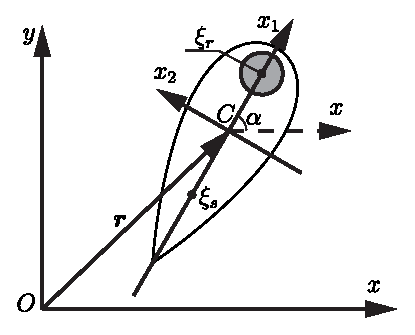
\includegraphics[width=0.4\linewidth]{coords.eps}
	\end{center}

	\item Две системы координат: неподвижная $Oxy$ и подвижная $Cx_1x_2$ жестко связанную с телом
	\item Радиус-вектор $\bs r = (x,\, y)$ точки $C$ определяет положение системы
	\item Угол $\alpha$ определяет ориентацию системы
	\item	Справедливы следующие кинематические соотношения:
	\begin{gather*}
	\begin{gathered}
	\dot{x} = v_1 \cos\alpha - v_2 \sin\alpha,\quad \dot{y} = v_1 \sin\alpha + v_2 \cos\alpha,\quad \dot{\alpha} = \omega,
	\end{gathered}
	\end{gather*}
\end{itemize}

\end{frame}


\begin{frame}
\frametitle{Математическая модель}

	\begin{itemize}
	
		%где $m$, $I$ --- масса и момент инерции робота соответственно, $f_1$, $f_2$ --- проекции силы реакции жидкости на подвижные оси, связанные с телом, $g$ --- момент силы реакции жидкости.
		\item Движение твердого тела в идеальной жидкости при нулевой циркуляции описывается уравнениями Кирхгофа. % их необходимо дополнить слагаемыми, описывающими вязкое трение \cite{Borisov_et_al_2016}:
		\begin{equation*}
		\begin{gathered}
		\der{}{t} \pder{T}{v_1} = \omega \pder{T}{v_2} - c_1 v_1 |v_1|,\quad \der{}{t} \pder{T}{v_2} = - \omega \pder{T}{v_1} - c_2 v_2 |v_2|,\\
		\der{}{t} \pder{T}{\omega} = v_2 \pder{T}{v_1} - v_1 \pder{T}{v_2} - c_3 \omega |\omega|,
		\end{gathered}\label{eq.kirchhoff}
		\end{equation*}
		где $T$ --- кинетическая энергия системы (корпус + ротор + жидкость), $c_1$, $c_2$, $c_3$ --- коэффициенты сопротивления.
		
		Кинетическая энергия системы с точностью до некоторой функции времени имеет вид
		\begin{gather*}
		T = \frac{1}{2}(m + \lambda_{11}) v_1^2 + \frac{1}{2}(m + \lambda_{22}) v_2^2 + \frac{1}{2} (I + \lambda_{33}) \omega^2 + \lambda_{23} v_2\omega + \omega k(t),\label{eq.T}\\
		\begin{gathered}
		m = m_s + m_r,\quad
		I = I_s + m_s \xi_s^2 + I_r + m_r \xi_r^2,\quad k(t) = I_r \Omega(t),
		\end{gathered}\notag
		\end{gather*}
	\end{itemize}

\end{frame}


\begin{frame}
\frametitle{Математическая модель}

\begin{itemize}
	\item Полная система уравнений рассматриваемой системы может быть записана в следующей форме:
	\begin{subequations}\label{eq.fullEqs}
		\begin{equation}
		\begin{split}\label{eq.dyn}
		(m + \lambda_{11}) \dot{v}_1 = {} & {} (m + \lambda_{22}) v_2 \omega + \lambda_{23}\omega^2 - c_1 v_1 |v_1|,\\
		(m + \lambda_{22}) \dot{v}_2 + \lambda_{23} \dot{\omega} = {} & {} - (m + \lambda_{11}) v_1 \omega - c_2 v_2 |v_2|,\\
		\lambda_{23}\dot{v}_2 + (I + \lambda_{33}) \dot{\omega} = {} & {} (\lambda_{11} - \lambda_{22}) v_1 v_2 - \lambda_{23} v_1\omega - c_3 \omega |\omega| - \dot{k}(t),
		\end{split}
		\end{equation}
		\begin{equation}
		\dot{x} = v_1 \cos\alpha - v_2 \sin\alpha,\quad \dot{y} = v_1 \sin\alpha + v_2 \cos\alpha,\quad \dot{\alpha} = \omega.
		\end{equation}
	\end{subequations}
	
	\item Уравнения Ньютона-Эйлера в подвижных осях, жестко связанных с телом:
	\begin{gather}
	\begin{gathered}
	m \dot{v}_1 = m v_2 \omega + f_1 (v_1,\, v_2,\, \omega,\, \dot{v}_1,\, \dot{v}_2,\, \dot \omega),\quad m \dot{v}_2 = -m v_1 \omega + f_2 (v_1,\, v_2,\, \omega,\, \dot{v}_1,\, \dot{v}_2,\, \dot \omega),\\
	I \dot{\omega} = g (v_1,\, v_2,\, \omega,\, \dot{v}_1,\, \dot{v}_2,\, \dot \omega),
	\end{gathered}\label{eq.NE}
	\end{gather}
	
	\item Сравнивая уравнения \eqref{eq.dyn} с уравнениями Ньютона-Эйлера \eqref{eq.NE}, запишем выражения для сил $f_1$, $f_2$ и момента $g$:
	\begin{gather}
	\begin{gathered}\label{eq.forceTorque}
	f_1 = - \lambda_{11}\dot{v}_1 + \lambda_{22} v_2 \omega + \lambda_{23}\omega^2 - c_1 v_1 |v_1|, \\
	f_2 = - \lambda_{22} \dot{v}_2 - \lambda_{23} \dot{\omega} - \lambda_{11} v_1 \omega - c_2 v_2 |v_2|,\\
	g = -\lambda_{23}\dot{v}_2 - \lambda_{33} \dot{\omega} + (\lambda_{11} - \lambda_{22}) v_1 v_2 - \lambda_{23} v_1\omega - c_3 \omega |\omega| - \dot{k}(t),
	\end{gathered}
	\end{gather}
	%где коэффициенты $\lambda_{ij}$ и $c_i$ подлежат определению, а $\dot{k}(t)$ --- определяется управляющим воздействием на ротор.
\end{itemize}

\end{frame}

\begin{frame}
\frametitle{Математическая модель}

\begin{itemize}
	\item Про уравнения Навье-Стокса...
	
	При известных распределениях $u_1$, $u_2$, $p$ cилы $f_1$, $f_2$ и момент $g$, действующие на тело со стороны жидкости, определяются следующими интегралами по контуру $L$ профиля:
	\begin{gather*}
	\begin{gathered}
	f_1 = \oint_L \left( p \pder{x_2}{\xi} + \frac{\rho \nu}{D} \pder{u_1}{\eta} \pder{x_1}{\xi} \right) d\xi,\\
	f_2 = \oint_L \left( -p \pder{x_1}{\xi} + \frac{\rho \nu}{D} \pder{u_1}{\eta} \pder{x_2}{\xi} \right) d\xi,\\
	g = \oint_L \left( x_1 \left( -p \pder{x_1}{\xi} + \frac{\rho \nu}{D} \pder{u_1}{\eta} \pder{x_2}{\xi} \right) - x_2 \left( p \pder{x_2}{\xi} + \frac{\rho \nu}{D} \pder{u_1}{\eta} \pder{x_1}{\xi} \right) \right) d\xi - \dot{k}(t).
	\end{gathered}\label{eq.fgNS}
	\end{gather*}
	
	\item \begin{gather}
	\begin{gathered}
	\lambda_{11}^{(1)} \approx 0.3087, \quad 
	\lambda_{22}^{(1)} \approx -0.5796,\quad 
	\lambda_{23}^{(1)} \approx 0.039085,\\
	\lambda_{22}^{(2)} \approx 2.0996,\quad 
	\lambda_{23}^{(2)} \approx 0.17629,\quad
	\lambda_{11}^{(2)} \approx -7.9826,\\
	\lambda_{23,l}^{(3)} \approx 0.083474,\quad
	\lambda_{33}^{(2)} \approx 0.018935,\quad
	\lambda_{11}^{(3)} - \lambda_{22}^{(3)} \approx - 4.7550,\quad
	\lambda_{23,r}^{(3)} \approx 1.4488,\\
	c_1 = 0.04715,\quad c_2 = 17.702,\quad c_3 = 0.092872.
	\end{gathered}\label{eq.coeffs2}
	\end{gather}
	
\end{itemize}

\end{frame}


\begin{frame}
\frametitle{Закон изменения угловой скорости ротора}



	\begin{itemize}
		\item В общем случае, зависимость угловой скорости ротора от времени будет иметь характерные переходные интервалы, соответствующие разгону и торможению 
	\end{itemize}
		\scriptsize 
		\begin{equation*}
		\omega_r(t) =
		\begin{cases}
		
		\omega_1 & t \in \left[ nT;  nT + t_1 \right] ,\\
		
		\frac{(\omega_2 - \omega_1)(t-nT)}{t_2} - \frac{(\omega_2 - \omega_1)(t_1+t_2)}{t_2} + \omega_2 & t \in \left[ nT + t_1;  nT + t_1+t_2 \right], \\
		
		\omega_2 & t \in \left[ nT + t_1+t_2;  nT + t_1+t_2+t_3 \right] ,\\
		
		\frac{(\omega_1 - \omega_2)(t-nT)}{t_4} - \frac{(\omega_1 - \omega_2)(t_1+t_2+t_3+t_4)}{t_4} + \omega_1 &t \in \left[ nT + t_1 + t_2+t_3;  nT + t_1+t_2+t_3+t_4 \right] ,
		
		\end{cases}
		\label{omegaRotorGeneral}
		\end{equation*}
		
		\small
		где $n \in \mathbf{N}$, $T$ -- период управляющего воздействия; $ \omega_1, \omega_2 $ -- амплитуды угловой скорости вращения ротора по часовой стрелке и против часовой стрелки соответственно; $t_1, t_2, t_3, t_4$ -- задают продолжительность по времени характерных интервалов угловой скорости вращения ротора. 
		
			%\framebreak
		
		Графически данная зависимость приведена на рисунке
		
		\begin{figure}[!ht]
			\centering
			\includegraphics[width=0.4\linewidth]{ControlAction.eps}
		\end{figure}
	
	
\end{frame}




\begin{frame}
\frametitle{Система управления}
Для управления безвинтовым недеформируемым рыбоподобным надводным роботом была разработана система управления, структурная схема которой представлена на рисунке

\begin{figure}[!h]
	\centering
	\includegraphics[width=0.8\linewidth]{ControlSystem.eps}
\end{figure}

\end{frame}

\begin{frame}
\frametitle{Экспериментальные исследования. Движение по прямой}
\begin{itemize}
	\item $t_1=t_3$, $ t_2 = t_4 \approx 0.1 $ секунды
	\item $ \omega_1 = \omega_{max} $, $ \omega_2 = -\omega_{max} $. 
	\item Таким образом, в качестве изменяемого параметра в экспериментах движения вдоль прямой выступает период $ T $, а $t_1=t_3 = 0.5(T - 2t_2)$. 
	Тогда функция $ \omega_r(t) $ примет вид 


\end{itemize}
\begin{figure}[!ht]
	\centering
	\includegraphics[width=0.5\linewidth]{ControlActionLine.eps}
\end{figure}

\end{frame}


\begin{frame}
\frametitle{Экспериментальные исследования. Движение по прямой}
\begin{figure}[!ht]
	\centering
	\includegraphics[width=1\linewidth]{AllTrajectories_new.eps}
\end{figure}

Траектории движения робота при  $ \omega_1 = \omega_{max} $, $ \omega_2 = -\omega_{max} $ и различных  управляющих воздействий, пунктирной линией обозначены траектории, полученные по результатам численного моделирования, сплошной - экспериментальные траектории.
\end{frame}


\begin{frame}
\frametitle{Экспериментальные исследования. Движение по прямой}
\begin{itemize}
	\item $ t_2=t_4=0.1 $ $ t_1=t_3=0.9 $, $T = 2$ с.
	\item Вращение ротора по часовой и против часовой стрелки с разными угловыми скоростями, при $ \omega_1 - \omega_2 = const$
	
	\begin{minipage}[h]{0.47\linewidth}
		Вид функции $ \omega_r(t) $ \\
		\center{\includegraphics[width=0.7\linewidth]{ControlActionPlots3.eps} \\ а)}
	\end{minipage}
	\hfill
	\begin{minipage}[h]{0.47\linewidth}
		Экспериментальные траектории движения робота
		\center{\includegraphics[width=0.7\linewidth]{Plots3.eps} \\ б)}
	\end{minipage}
	
	
	
	
	
\end{itemize}


\end{frame}


%\begin{frame}
%\frametitle{Экспериментальные исследования. Движение по прямой}
%\begin{figure}[!ht]
%\centering
%\includegraphics[width=0.5\linewidth]{Plots3.eps}
%\end{figure}
%
%Экспериментальные траектории движения робота при $ \omega_1 - \omega_2 = const$ 
%\end{frame}


\begin{frame}
\frametitle{Движение по прямой. Выводы}
	\begin{itemize}
		\item Рассматриваемая теоретическая модель управляемого движения водного робота качественно правильно  описывает его движение вдоль прямой, которое реализуется симметричным управляющим воздействием.
		\item Сдвиг управляющего воздействия $\omega(t) \rightarrow \omega_0 + \omega(t)$ не влияет на форму траектории, она остается прямой, но меняется направление движение.
		\item Количественного согласования результатов моделирования и экспериментов можно достичь для конкретных тестов, проводя перерасчет коэффициентов под конкретные экспериментальные данные.
	\end{itemize}
	
\end{frame}


\begin{frame}
\frametitle{Экспериментальные исследования. Движение по окружности}
	\begin{itemize}
		\item $t_1 \neq t_3$, $t_2 = t_4$ с.
		\item $ \omega_1 = \omega_{max} $, $ \omega_2 = -\omega_{max} $. 
		\item $ k_1 = t_3 / t_1 $
	\end{itemize}
		
	 \begin{minipage}[t]{0.47\linewidth}
		{Зависимость угловой скорости ротора от времени \\}
		\center{\includegraphics[width=1\linewidth]{ControlActionCircle.eps}}
	\end{minipage}
	\hfill
	\begin{minipage}[t]{0.47\linewidth}
		{Траектория движения робота по окружности при эксперименте (штриховая линия) и моделировании (сплошная линия)}
		\center{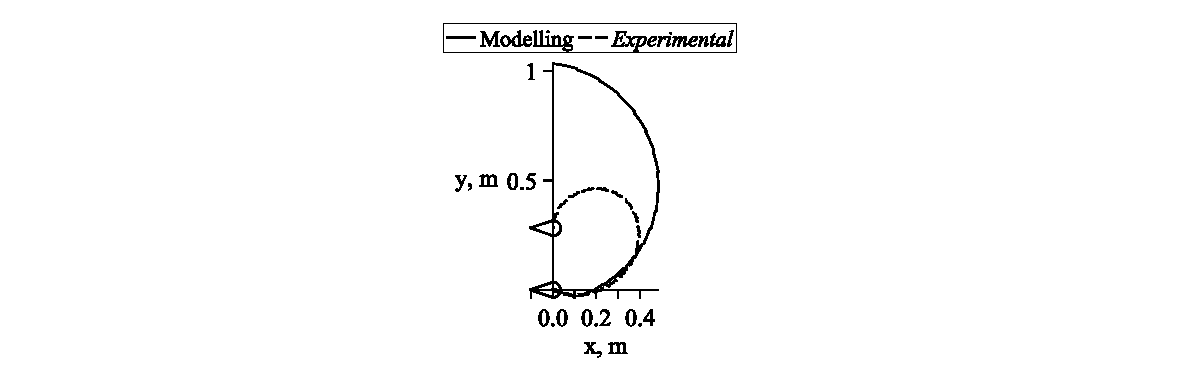
\includegraphics[width=0.5\linewidth]{xyCircleWmax.eps}}
	\end{minipage}

\end{frame}





\begin{frame}
\frametitle{Экспериментальные исследования. Движение по окружности}
\begin{itemize}
	\item $t_1 = t_3$, $t_2 \neq t_4$ с.
	\item $ \omega_1 = \omega_{max} $, $ \omega_2 = -\omega_{max} $. 
	\item $ k_2 = t_2 / t_4 $
\end{itemize}

\begin{minipage}[t]{0.47\linewidth}
	{Зависимость угловой скорости ротора от времени \\}
	\center{\includegraphics[width=1\linewidth]{ControlActionOur1.eps}}
\end{minipage}
\hfill
\begin{minipage}[t]{0.47\linewidth}
	{Траектория движения робота по окружности при эксперименте (штриховая линия) и моделировании (сплошная линия)}
	\center{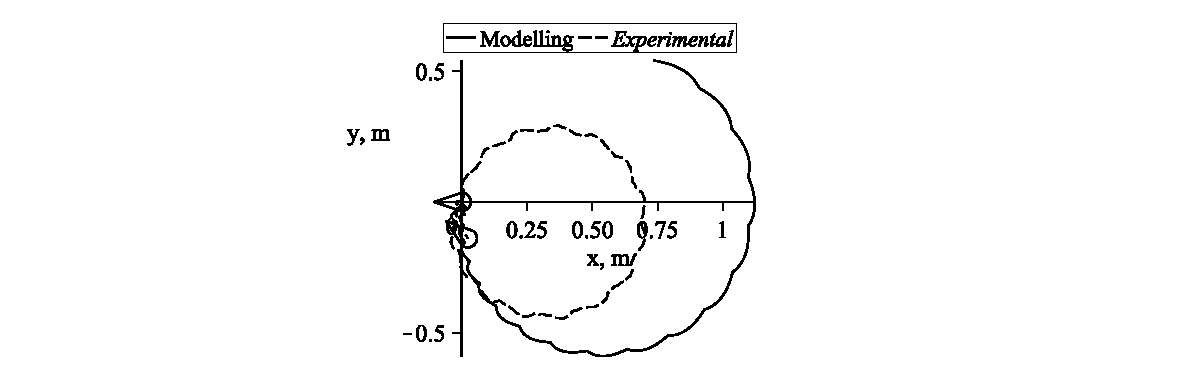
\includegraphics[width=0.7\linewidth]{xyCircleOur.eps}}
\end{minipage}

\end{frame}

\begin{frame}
\frametitle{Экспериментальные исследования. Движение по окружности}

%{Зависимость радиуса траектории движения робота от $k_1 = \frac{t_3}{t_1}$ при эксперименте (штриховая линия) и моделировании (сплошная линия) построенная по экспериментам при $k_1 = 2, 3, 5, 10$}
%\center{\includegraphics[width=0.9\linewidth]{kRDependence+Theor_T=3,W=max.eps}}

\begin{minipage}[t]{0.47\linewidth}
	{Зависимость радиуса траектории движения робота от $k_1 = \frac{t_3}{t_1}$ при эксперименте (штриховая линия) и моделировании (сплошная линия) построенная по экспериментам при $k_1 = 2, 3, 5, 10$}
	\center{\includegraphics[width=0.9\linewidth]{kRDependence+Theor_T=3,W=max.eps}}
\end{minipage}
\hfill
\begin{minipage}[t]{0.47\linewidth}
	{Зависимость радиуса траектории движения робота от $k_2 = \frac{t_2}{t_4}$ при эксперименте (штриховая линия) и моделировании (сплошная линия) построенная по экспериментам при $k_2 = 10, 20, 30, 40$}
	\center{\includegraphics[width=1.05\linewidth]{nROur.eps}}
\end{minipage}

\end{frame}

%\begin{frame}
%\frametitle{Экспериментальные исследования. Движение по окружности}
%{Зависимость радиуса траектории движения робота от $k_2 = \frac{t_2}{t_4}$ при эксперименте (штриховая линия) и моделировании (сплошная линия) построенная по экспериментам при $k_2 = 10, 20, 30, 40$}
%\center{\includegraphics[width=0.9\linewidth]{nROur.eps}}
%\end{frame}

\begin{frame}
\frametitle{Движение по окружности. Выводы}
\begin{itemize}
	\item Рассматриваемая теоретическая модель управляемого движения водного робота качественно правильно  описывает его движение вдоль окружности, которое реализуется асимметричным на периоде управляющим воздействием.
	\item На размер и форму траектории движения влияет асимметрия управляющего воздействия на его периоде. Изменение направления движения -- поворот, может быть реализован либо при изменении продолжительности интервала вращения с постоянной угловой скоростью, либо вращением ротора по и против часовой стрелки с различными угловыми ускорениями.
	\item Количественного согласования результатов моделирования и экспериментов, как и в при движении вдоль прямой, можно достичь для конкретных тестов, проводя перерасчет коэффициентов под конкретные экспериментальные данные, полученные при движении вдоль окружности.
\end{itemize}

\end{frame}


\begin{frame}
\frametitle{Экспериментальные исследования. Движение вдоль сложных траекторий}


	{Управления для слалома}
	\centering
	\includegraphics[width=0.7\linewidth]{ControlActionComplexTr.eps}

	{Траектория движения робота при эксперименте (штриховая линия) и моделировании (сплошная линия)}
	\centering
	\includegraphics[width=0.7\linewidth]{ComplexTr.eps}


\end{frame}

\begin{frame}
\frametitle{Экспериментальные исследования. Видео.}


%\movie[width=0.5\textwidth]{\includegraphics[width=0.5\textwidth]{ComplexTr1.png}}{123.mp4}
%\includemedia[activate=onclick, width=0.5\textwidth]{\includegraphics{ComplexTr1.png}}{123.mp4}
%\includemedia[
%activate=pageopen,
%width=1280pt,height=720pt,
%addresource=123.mp4,
%flashvars={
%	source=123.mp4}
%]{}{VPlayer.swf}

\end{frame}



\begin{frame}
\frametitle{Заключение}
\begin{itemize}
	\item Адекватность математической модели.
	\item Основная причина отклонения результатов моделирования -- рассчет коэффициентов модели на основании экспериментальных  данных, полученных при симметричном управляющем воздействии с $T = 1 $ c.
	\item Вторая причина несогласованности теории и эксперимента -- не точное совпадение формы углового ускорения в моделировании и при эксперименте.
\end{itemize}

Зависимость угловой скорости ротора и углового ускорения ротора от времени при эксперименте (штриховая линия) и моделировании (сплошная линия)

\begin{minipage}[t]{0.47\linewidth}
	\center{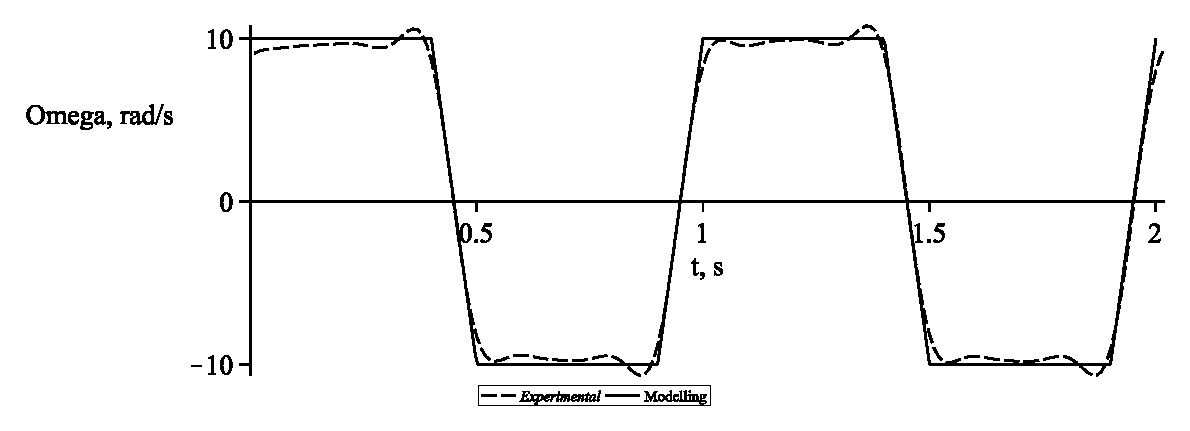
\includegraphics[width=1\linewidth]{OmegaT1Meandr.eps}}
\end{minipage}
\hfill
\begin{minipage}[t]{0.47\linewidth}
	\center{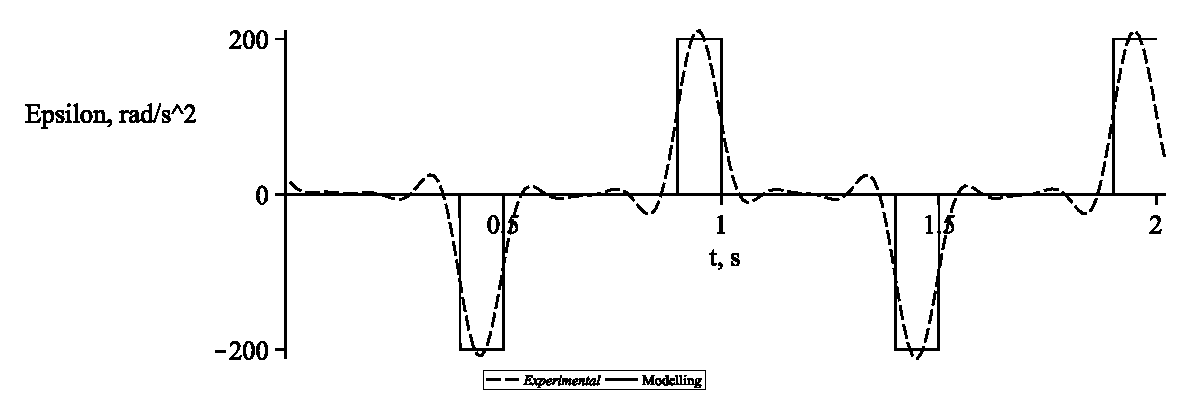
\includegraphics[width=1\linewidth]{EpsilonT1Meandr.eps}}
\end{minipage}

\end{frame}

%%%%%%%%%%%%%%%%%%%%%%%%%%%%%%%%%%%%%%%%%%%%%%%%%%%%%%%%%%%%%%%%%%%%%%%%%%%%%%%%%%%%%%%%%%%%
%\section{Списки}
%\begin{frame}[plain, noframenumbering]
%    \begin{center}
%        \Huge
%        Списки
%    \end{center}
%\end{frame}
%
%\subsection{Нумерованные}
%
%\begin{frame}
%    \frametitle{Нумерованные списки}
%    \begin{enumerate}
%        \item один
%        \item два
%        \item три
%    \end{enumerate}
%\end{frame}
%\note{
%    Этот текст будет виден только если его отображение включено в файле \textbf{Presentation/setup}.
%    Для раздельного вывода презентации и заметок на разные экраны (как в impress или powerpoint) можно использовать программу \textit{pdf-presenter-console}.
%}
%
%\subsection{Не нумерованные}
%
%
%\begin{frame}
%    \frametitle{Перечисления}
%    \begin{itemize}
%        \item Проблема 1
%        \item Проблема 2
%        \item Проблема 3
%    \end{itemize}
%\end{frame}
%\note[itemize]{
%    \item Тезис 1
%    \item Тезис 2
%    \item Тезис 3
%}
%
%\subsection{Комбинированные}
%
%\begin{frame}
%    \frametitle{Комбинация списков}
%    \begin{enumerate}
%        \item \textbf{Задача 1}
%              \begin{itemize}
%                  \item Подзадача 1-1
%                  \item Подзадача 1-2
%              \end{itemize}
%        \item \textbf{Задача 2}
%              \begin{itemize}
%                  \item Подзадача 2-1
%                  \item Подзадача 2-2
%                  \item Подзадача 2-3
%              \end{itemize}
%        \item \textbf{Задача 3}
%              \begin{itemize}
%                  \item Подзадача 3-1
%                  \item Подзадача 3-2
%                  \item Подзадача 3-3
%              \end{itemize}
%    \end{enumerate}
%\end{frame}
%\note[itemize]{
%    \item Задача 1
%    \item Задача 2
%    \item Задача 3
%}
%
%\begin{frame}[allowframebreaks]
%    \frametitle{Разделение слайда}
%    Поясняющий текст
%    \begin{itemize}
%        \item Один
%        \item Два
%        \item Три
%    \end{itemize}
%    \framebreak
%    Продолжение предыдущего слайда
%\end{frame}
%
%\section{Графика}
%\begin{frame}[plain, noframenumbering]
%    \begin{center}
%        \Huge
%        Графика
%    \end{center}
%\end{frame}
%
%
%\begin{frame}
%    \frametitle{Одиночное изображение}
%    \centering
%    \includegraphics[width=0.8\linewidth]{latex} % окружение figure не требуется
%\end{frame}
%
%\begin{frame}
%    \frametitle{Векторная графика}
%    \begin{figure}
%	    \centering
%	    \ifdefmacro{\tikzsetnextfilename}{\tikzsetnextfilename{tikz_presentation}}{}% присваиваемое предкомпилированному pdf имя файла (не обязательно)
%	    \input{Presentation/images/tikz_plot.tikz}
%    \end{figure}
%\end{frame}
%
%\subsection{Расположение}
%
%\begin{frame}
%    \frametitle{Изображения по-вертикали}
%    \centering
%    \vfill
%    \includegraphics[width=0.8\linewidth,height=0.1\textheight]{latex} \\
%    \TeX
%    \vfill
%    \includegraphics[width=0.8\linewidth,height=0.2\textheight]{latex} \\
%    \LaTeX
%    \vfill
%    \includegraphics[scale=0.2]{latex} \\
%    \vfill
%\end{frame}
%
%
%\begin{frame}
%    \frametitle{Изображения по-горизонтали}
%    \begin{minipage}[t]{0.47\linewidth}
%        \textbf{Составная \\ подпись 1}
%        \center{\includegraphics[width=1\linewidth]{knuth1}}
%    \end{minipage}
%    \hfill
%    \begin{minipage}[t]{0.47\linewidth}
%        \textbf{Составная \\ подпись 2}
%        \center{\includegraphics[width=1\linewidth]{knuth2}}
%    \end{minipage}
%\end{frame}
%
%\subsection{Линии}
%
%\begin{frame}
%    \frametitle{Разделяющие линии}
%    \begin{minipage}[c]{0.47\linewidth}
%        \center{\includegraphics[width=1\linewidth]{latex}}
%        \bigskip
%        \hrule{}
%        \bigskip
%        \textbf{Составная \\ подпись 1}
%    \end{minipage}
%    \hfill
%    \vrule{}
%    \hfill
%    \begin{minipage}[c]{0.47\linewidth}
%        \flushright
%        \textbf{Составная \\ подпись 2}
%        \center{\includegraphics[width=1\linewidth]{knuth2}}
%    \end{minipage}
%\end{frame}
%
%\section{Остальное}
%\begin{frame}[plain, noframenumbering]
%    \begin{center}
%        \Huge
%        Остальное
%    \end{center}
%\end{frame}
%
%\subsection{Формулы}
%
%\begin{frame}
%    \frametitle{Формулы}
%    \[
%    \left\{
%    \begin{array}{rl}
%        \dot x = & \sigma (y-x)  \\
%        \dot y = & x (r - z) - y \\
%        \dot z = & xy - bz
%    \end{array}
%    \right.
%    \]
%\end{frame}
%
%\begin{frame}
%    \frametitle{amsmath}
%    \centering
%    \begin{minipage}[t]{0.5\linewidth}
%        \begin{multline*}
%            y = 1 x^1 + 2 x^2 + 3 x^3 + \\ + 4 x^4 + 5 x^5 + \dots
%        \end{multline*}
%    \end{minipage}
%\end{frame}
%
%\begin{frame}[allowframebreaks]
%    \frametitle{Уравнения Максвелла}
%    \centering{
%        \small
%        \def\arraystretch{1.8}%
%        \begin{tabular}{ll}
%            \toprule
%            Интегральная форма                                                                                                                                          & Дифференциальная форма                                                        \\ \midrule
%            \(Q_e(t) = \displaystyle\oiint_S \vec D(t) \cdot d\vec{s} = \displaystyle\iiint_V \rho_v(t) dv\)                                                              & \(\nabla \cdot \vec D(t) = \rho_v(t)\)                                          \\
%            \(\displaystyle\oiint_S \vec B(t) \cdot d\vec{s} = 0\)                                                                                                        & \(\nabla \cdot \vec B(t) = 0\)                                                  \\
%            \(V_{emf}(t) = \displaystyle\oint_L \vec E(t) \cdot d\vec{l}\) = \(- \displaystyle\iint_S \left[\frac{\partial\vec{B}(t)}{\partial t}\right] \cdot d\vec{s}\)   & \(\nabla \times \vec E(t) = - \frac{\partial\vec{B}(t)}{\partial t}\)           \\
%            \(I(t) = \displaystyle\oint_L \vec H(t) \cdot d\vec{l} = \displaystyle\iint_S \left[\vec J(t) + \frac{\partial\vec{D}(t)}{\partial t}\right] \cdot d\vec{s}\) & \(\nabla \times \vec H(t) = \vec J(t) + \frac{\partial\vec{D}(t)}{\partial t}\) \\ \midrule
%            \(\displaystyle\oiint_S \vec J \cdot d\vec{s} = -\frac{\partial Q_e}{\partial t}\)                                                                            & \(\nabla \cdot \vec J = - \frac{\partial \rho_v}{\partial t}\)                  \\
%            \bottomrule
%            \multicolumn{2}{c}{\(\vec D(t) = \left[\varepsilon(t)\right] * \vec E(t)\)}                                                                                                                                                                   \\
%            \multicolumn{2}{c}{\(\vec B(t) = \left[\mu(t)\right] * \vec H(t)\)}                                                                                                                                                                           \\
%        \end{tabular}
%    }
%    \framebreak
%
%    \hspace{0.05\linewidth}
%    \centering{
%        \small
%        \def\arraystretch{1.8}%
%        \begin{tabular}{ll}
%            \toprule
%            Интегральная форма                                                                                                            & Дифференциальная форма                             \\ \midrule
%            \(Q_e = \displaystyle\oiint_S \vec D \cdot d\vec{s} = \displaystyle\iiint_V \rho_v dv\)                                         & \(\nabla \cdot \vec D = \rho_v\)                     \\
%            \(\displaystyle\oiint_S \vec B \cdot d\vec{s} = 0\)                                                                             & \(\nabla \cdot \vec B = 0\)                          \\
%            \(V_{emf} = \displaystyle\oint_L \vec E \cdot d\vec{l}\) = \(- \displaystyle\iint_S \left[j \omega \vec B\right] \cdot d\vec{s}\) & \(\nabla \times \vec E = - j \omega \vec B\)         \\
%            \(I = \displaystyle\oint_L \vec H \cdot d\vec{l} = \displaystyle\iint_S \left[\vec J + j \omega \vec D\right] \cdot d\vec{s}\)  & \(\nabla \times \vec H = \vec J + j \omega \vec{D}\) \\ \midrule
%            \(\displaystyle\oiint_S \vec J \cdot d\vec{s} = - j \omega Q_e\)                                                                & \(\nabla \cdot \vec J = - j \omega \rho_v\)          \\
%            \bottomrule
%            \multicolumn{2}{c}{\(\vec D(t) = \left[\varepsilon\right] \vec E(t)\)}                                                                                                               \\
%            \multicolumn{2}{c}{\(\vec B(t) = \left[\mu\right] \vec H(t)\)}                                                                                                                       \\
%        \end{tabular}
%    }
%\end{frame}
%
%\subsection{Таблицы}
%
%\begin{frame}
%    \frametitle{Таблица}
%    \centering
%    \begin{tabular}{|l|l|}
%        \hline
%        \textbf{Заголовок 1} & \textbf{Заголовок 2} \\
%        \hline
%        Сумма                & \(b+a\)                \\
%        \hline
%        Разность             & \(a-b\)                \\
%        \hline
%        Произведение         & \(a*b\)                \\
%        \hline
%    \end{tabular}
%\end{frame}
%
%\begin{frame}
%    \frametitle{Другая таблица}
%    \centering
%    \begin{tabular}{lc}
%        \toprule
%        \multicolumn{1}{c}{\textbf{Заголовок 1}} & \textbf{Заголовок 2} \\ \midrule
%        Сумма                                    & \(b+a\)                \\
%        Разность                                 & \(a-b\)                \\
%        Произведение                             & \(a*b\)                \\
%        \bottomrule
%    \end{tabular}
%\end{frame}
%
%
%\subsection{Разное}
%
%\begin{frame}
%    \frametitle{Большой многоуровневый список}
%    \begin{itemize}
%        \item \textbf{Пункт 1}
%              \begin{itemize}
%                  \itemi Подпункт 1-1
%                  \itemi Подпункт 1-2
%              \end{itemize}
%        \item \textbf{Пункт 2}
%              \begin{itemize}
%                  \itemi Подпункт 2-1
%              \end{itemize}
%        \item \textbf{Пункт 3}
%              \begin{itemize}
%                  \itemi Подпункт 3-1
%                  \itemi Подпункт 3-2
%              \end{itemize}
%        \item \textbf{Пункт 4}
%              \begin{itemize}
%                  \itemi Подпункт 4-1
%              \end{itemize}
%        \item \textbf{Пункт 5}
%              \begin{itemize}
%                  \itemi Подпункт 5-1
%                  \itemi Подпункт 5-2
%                  \itemi Подпункт 5-3
%              \end{itemize}
%    \end{itemize}
%\end{frame}
%
%\begin{frame}
%    \frametitle{Четыре изображения}
%    \centering
%    \includegraphics[width=0.35\linewidth,angle=35]{latex}
%    \includegraphics[width=0.35\linewidth,angle=135]{latex}\\
%    \includegraphics[width=0.35\linewidth,angle=15]{latex}
%    \includegraphics[width=0.35\linewidth,angle=-15]{latex}
%\end{frame}

